% !TeX root = mos-en.tex

%%%%%%%%%%%%%%%%%%%%%%%%%%%%%%%%%%%%%%%%%%%%%%%%%%%%%%%%%%%%%%%%

\refstepcounter{problem}  % 41. The locomotive problem

%%%%%%%%%%%%%%%%%%%%%%%%%%%%%%%%%%%%%%%%%%%%%%%%%%%%%%%%%%%%%%%%

\begin{prob}{The little end of the stick\annotate{S}}
A large number of glass rods each of length $1$ are broken into two pieces each. The breaking point is uniformly distributed along the lengths of the rods.

\que{1} What is the expectation of the length of the \emph{smaller} piece?

\que{2} What is the expectation of the ratio of the length of the smaller piece to the larger piece?
\end{prob}
\solution{}

\ans{1} The probability that the break is on the left half of a rod is $1/2$ as is the probability that it is on the right half.
The smaller piece is on the same side as the break so the expectation of its position is halfway between the end and the middle:
\[
E(\textsf{length of smaller piece}) = \frac{1}{2}\cdot\frac{1}{2}=\frac{1}{4}\,.
\]

\ans{2} Without loss of generality assume that the break occurred in the right half of the rod (Figure~\ref{f.stick}). The ratio of the smaller piece to the larger piece is $(1-x)/x$ and the length of the larger piece $x$ is uniformly distributed in $(1/2,1)$. Therefore:
\begin{eqn}
E(\textsf{ratio of smaller to larger})&=&\left(\frac{1}{1-(1/2)}\right)\int_{1/2}^1 \frac{1-x}{x} \,dx\\
&=& 2\int_{1/2}^1 \left(\frac{1}{x} -1\right) \,dx \\
&=& 2\left.(\ln |x| - x)\right|_{1/2}^1 = 2\ln 2 -1\approx 0.3863\,.
\end{eqn}
\begin{figure}[tb]
\begin{center}
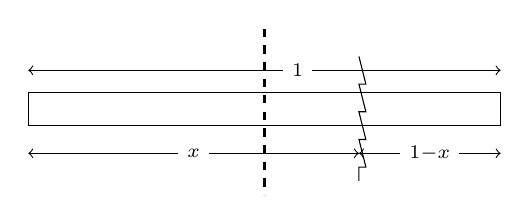
\begin{tikzpicture}
\draw (0,0) -- ++(6,0) -- ++(0,12pt) -- ++(-6,0) -- cycle;
\draw[<->] (0,20pt) --
  node[fill=white,xshift=12pt] {$\scriptstyle 1$} ++(6,0);
\draw[decorate,decoration=saw] (4.2,25pt) -- +(0,-45pt);
\draw[thick,dashed] (3,35pt) -- +(0,-60pt);
\draw[<->] (0,-10pt) --
  node[fill=white] {$\scriptstyle x$} (4.2,-10pt);
\draw[<->] (4.2,-10pt) --
  node[fill=white] {$\scriptstyle 1-x$} (6,-10pt);
\end{tikzpicture}
\end{center}
\caption{Breaking a stick into two pieces}\label{f.stick}
\end{figure}

\textbf{Simulation}
\begin{verbatim}
Expectation of length of smaller = 0.2500
Average length of smaller        = 0.2490
Expectation of smaller/larger    = 0.3863
Average smaller/larger           = 0.3845
\end{verbatim}

%%%%%%%%%%%%%%%%%%%%%%%%%%%%%%%%%%%%%%%%%%%%%%%%%%%%%%%%%%%%%%%%


\begin{prob}{The broken bar\annotate{D,S}}

A large number of glass rods of length $1$ are broken in two places (Figure~\ref{f.break1}).

\que{1} What is the expectaton of the length of the shortest piece?

\que{2} What is the expectaton of the length of the longest piece?

\textbf{Hint:} $x,y$ are independent random variables with a uniform distribution from $(0,1)$. Each pair $(x,y)$ can be represented as a point in the unit square $(0,1)\times (0,1)$ (Figure~\ref{f.break2}). What is the probability that $(x,y) < (.5,.25)$? 

\textbf{Hint:} For \que{1} assume that left piece is the shortest one and for \que{2} assume that the left piece is the longest one.
\begin{figure}[tb]
\begin{center}
\begin{subfigure}{.4\textwidth}
\begin{tikzpicture}[scale=.75]
\draw (0,0) node[below left] {$0$} --
  ++(6,0) node[below right] {$1$} --
  ++(0,12pt) -- ++(-6,0) -- cycle;
\draw[<->] (0,20pt) --
  node[fill=white] {$\scriptstyle 1$} ++(6,0);
\draw[decorate,decoration=saw] (1.8,25pt) -- +(0,-45pt);
\draw[decorate,decoration=saw] (4.7,25pt) -- +(0,-45pt);
\node[below left] at (1.8,0) {$x$};
\node[below left] at (4.7,0) {$y$};
\path (0,-3.5) rectangle +(0,3.5);
\end{tikzpicture}
\caption{Break a rod into two pieces\hspace{6em}\mbox{}}\label{f.break1}
\end{subfigure}
\hspace{3em}
\begin{subfigure}{.4\textwidth}
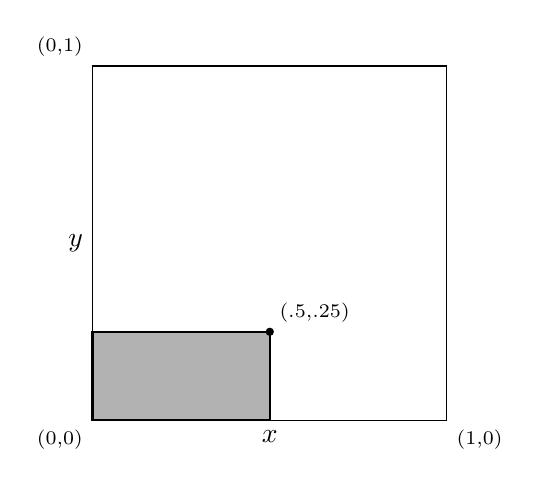
\begin{tikzpicture}[scale=.75]
\draw (-3,-3) rectangle +(6,6);
\draw[thick,fill=white!70!black] (-3,-3) -- ++(0,1.5) -- 
  ++(3,0) -- ++(0,-1.5) -- cycle;
\path (-3,-3) node[below left] {$\scriptstyle (0,0)$} --
  node[below] {$x$} (3,-3)
  node[below right] {$\scriptstyle (1,0)$};
\path (-3,-3) -- node[left] {$y$} (-3,3)
  node[above left] {$\scriptstyle (0,1)$};
\fill (0,-1.5) circle [radius=2pt]
  node[above right] {$\scriptstyle (.5,.25)$};
\end{tikzpicture}
\caption{Representation of the lengths in the unit square}\label{f.break2}
\end{subfigure}
\end{center}
\end{figure}
\end{prob}
\solution{}

\ans{1} Without loss of generality assume that the left piece of length $x$ is the shortest. Then $x<y-x$ and $x < 1-y$, from which we have $2x<y$ and $x+y<1$.

Figure~\ref{f.shaded1} shows the lines $y=2x$ (red) and $y=1-x$ (blue).  For the inequalities to be true, $(x,y)$ must be in the shaded region left of the two lines. The point of intersection $(1/2,2/3)$ can be computed by solving the two equations.

While the values of $(x,y)$ are in the square $(0,1)\times(0,1)$, the expectation is computed over the shaded subset of the square so the integral must be divided by the area of the shaded region: $\frac{1}{2} (\frac{1}{3}\cdot 1)=\frac{1}{6}$:
\begin{eqn}
E(x)&=& \frac{1}{1/6}\int_{0}^{1/3} x [(1-x)-2x]\,dx\\
&=&\int_{0}^{1/3} (6x -18x^2)\,dx\\
&=&\left. (3x^2-6x^3)\right|_0^{1/3}=\disfrac{2}{18}\approx 0.1111\,.
\end{eqn}

\begin{figure}[tb]
\begin{center}
\begin{subfigure}{.46\textwidth}
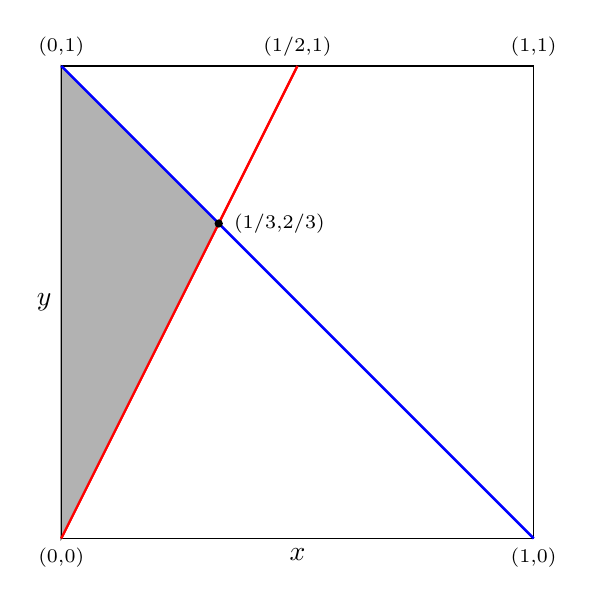
\begin{tikzpicture}[scale=1]
\draw (-3,-3) rectangle +(6,6);
\path (-3,-3) node[below] {$\scriptstyle (0,0)$} --
  node[below] {$x$} (3,-3)
  node[below] {$\scriptstyle (1,0)$};
\path (-3,-3) -- node[left] {$y$} (-3,3)
  node[above] {$\scriptstyle (0,1)$};
\draw[red,thick]  (-3,-3) -- (0,3);
\draw[blue,thick] (-3,3)  -- (3,-3);
\coordinate (P) at (-1,1);
\draw[fill=white!70!black] (-3,-3) -- (P) -- 
  (-3,3) -- cycle;
\draw[red,thick]  (-3,-3) -- (0,3);
\draw[blue,thick] (-3,3)  -- (3,-3);
\fill (P) circle[radius=1.5pt]
  node[right,xshift=2pt] {$\scriptstyle (1/3,2/3)$};
%\draw[thick,dotted] (-3,-3) -- (3,3);
\node[above] at(0,3) {$\scriptstyle (1/2,1)$};
\node[above] at(3,3) {$\scriptstyle (1,1)$};
\end{tikzpicture}
\caption{Shaded area for shortest bar}\label{f.shaded1}
\end{subfigure}
\hspace{1em}
\begin{subfigure}{.46\textwidth}
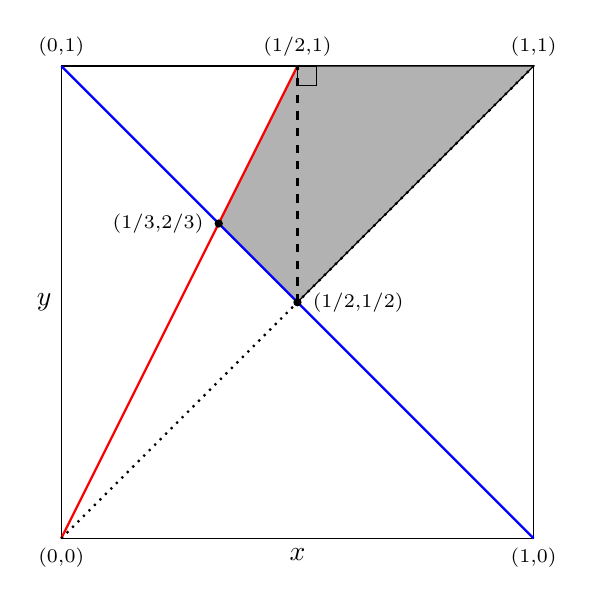
\begin{tikzpicture}[scale=1]
\draw (-3,-3) rectangle +(6,6);
\path (-3,-3) node[below] {$\scriptstyle (0,0)$} --
  node[below] {$x$} (3,-3)
  node[below] {$\scriptstyle (1,0)$};
\path (-3,-3) -- node[left] {$y$} (-3,3)
  node[above] {$\scriptstyle (0,1)$};
\coordinate (P) at (-1,1);
\coordinate (Q) at (0,0);
\draw[fill=white!70!black] (3,3) -- (Q) -- 
  (P) -- (0,3) -- cycle;
\draw[red,thick]  (-3,-3) -- (0,3);
\draw[blue,thick] (-3,3)  -- (3,-3);
\fill (P) circle[radius=1.5pt]
  node[left,xshift=-2pt] {$\scriptstyle (1/3,2/3)$};
\draw[thick,dotted] (-3,-3) -- (3,3);
\fill (Q) circle[radius=1.5pt]
  node[right,xshift=2pt] {$\scriptstyle (1/2,1/2)$};
\node[above] at(0,3) {$\scriptstyle (1/2,1)$};
\node[above] at(3,3) {$\scriptstyle (1,1)$};
\draw[thick,dashed] (Q) -- ++(0,3);
\draw (0,3cm-7pt) rectangle +(7pt,7pt);
\end{tikzpicture}
\caption{Shaded area for longest bar}\label{f.shaded2}
\end{subfigure}
\end{center}
\end{figure}

\ans{2}
For the left piece to be the longest, $x>y-x$ and $x>1-y$, so
$(x,y)$ must lie to the right of $y=2x$ (red) and to the right of $y=1-x$ (blue) (Figure~\ref{f.shaded2}). Furthermore, by the assumption that $x$ is to the left of $y$, $(x,y)$ must lie to the left of $y=x$ (dotted).

For convenience we divide the shaded region into two triangles (dashed line) and compute the expectations separately. The area of the shaded region is the sum of the areas of the triangles $1/24+1/8=1/6$. Then:
\begin{eqn}
E(x \textsf{\ in left triangle})&=& 6\int_{1/3}^{1/2} x [2x-(1-x)]\,dx  \\
&=&\int_{1/3}^{1/2} \left(18x^2-6x\right)\,dx\\
&=&\left. (6x^3-3x^2)\right|_{1/3}^{1/2}=\disfrac{1}{9}\\
E(x \textsf{\ in right triangle})&=& 6\int_{1/2}^{1} x [1-x]\,dx\\
&=&\int_{1/2}^{1} (6x-6x^2)\,dx\\
&=&\left. \left(3x^2-2x^3\right)\right|_{1/2}^{1}= \disfrac{1}{2}\\
E(x)&=& \disfrac{1}{9}+\disfrac{1}{2} = \disfrac{11}{18}\approx 0.6111\,.
\end{eqn}

The expectation of the length of the middle-sized piece is $1-\frac{2}{18}-\frac{11}{18}=\frac{5}{18}\approx 0.2778$.

\textbf{Simulation}
\begin{verbatim}
Expectations: shortest = 0.1111, middle = 0.2778, longest = 0.6111
Averages:     shortest = 0.1115, middle = 0.2783, longest = 0.6102
\end{verbatim}

%%%%%%%%%%%%%%%%%%%%%%%%%%%%%%%%%%%%%%%%%%%%%%%%%%%%%%%%%%%%%%%%

\begin{prob}{Winning an unfair game\annotate{D,S}}
You are given an unfair coin whose probability of heads is $1/3 < p < 1/2$. Toss a coin an even number of times $N=2n$. You win if and only \emph{more} than half of the tosses are heads.

\que{1} Develop a formula for the probability $P_N$ of winning and develop a formula for the probability $T_N$ of a tie occurring.

\que{2} Develop a formula for the $N$ that gives the highest probability of winning.

\textbf{Hint:} If $N$ tosses gives the highest probability of winning then $P_{N-2} \leq P_N$ and $P_N\geq P_{N+2}$.
\end{prob}
\solution{}

\ans{1} To win, heads needs to appear in $i\in\{n+1, n+2, \ldots, 2n-1, 2n=N\}$ tosses. From the binomial distribution:
\begin{eqn}
P_N &=& \sum_{i=n+1}^{2n} \dischoose{2n}{i} p^i (1-p)^{2n-i}\\
T_N &=& \dischoose{2n}{n} p^n (1-p)^{n}\,.
\end{eqn}

\ans{2} For $N=2n$ to give the highest probability of winning we must have:
\[
P_{2n-2} \leq P_{2n} \quad \textsf{and} \quad P_{2n}\geq P_{2n+2}\,.
\]
When is $P_{2n-2}\not = P_{2n}$?

\textit{Case 1:}
After toss $2n-2$, heads has appeared $n$ times and tails  $n-2$ times (so you would have won if you stop here), but tails appears in the next two tosses. You now have $n$ heads and $n$ tails, and therefore you lose. The probability is:
\[
\dischoose{2n-2}{n}p^n(1-p)^{n-2} (1-p)^2\,.
\]

\textit{Case 2:}
After toss $2n-2$, heads has appeared $n-1$ times and tails $n-1$ times (so you would have lost if you stop here), but heads appears in the next two tosses. You now have $n+1$ heads and $n-1$ tails and therefore you win. The probability is:
\[
\dischoose{2n-2}{n-1}p^{n-1}(1-p)^{n-1} p^2\,.
\]
For $P_{2n-2}\leq P_{2n}$ to hold $P_{2n-2}$ cannot increase while $P_{2n}$ remains the same (Case 1), although $P_{2n}$ can become greater than $P_{2n-2}$ (Case 2). Therefore:
\begin{eqn}
\dischoose{2n-2}{n}p^n(1-p)^{n-2} (1-p)^2 &\leq&
\dischoose{2n-2}{n-1}p^{n-1}(1-p)^{n-1} p^2\\
\disfrac{1}{n} (1-p) &\leq& \disfrac{1}{n-1} p\\
(n-1)(1-p) &\leq& np\\
n &\leq& \disfrac{1-p}{1-2p}\\
2n &\leq& \disfrac{1}{1-2p}+1\,.
\end{eqn}
Similarly, for $P_{2n}\geq P_{2n+2}$ to hold it must be true that:
\begin{eqn}
\dischoose{2n}{n+1}p^{n+1}(1-p)^{n-1}  (1-p)^2 &\geq&
\dischoose{2n}{n}p^{n}(1-p)^{n}  p^2\\
\disfrac{1}{n+1} (1-p) &\geq& \disfrac{1}{n} p\\
n(1-p)&\geq& (n+1)p\\
n &\geq& \disfrac{p}{1-2p}\\
2n &\geq&\disfrac{1}{1-2p}-1\,.
\end{eqn}
Therefore, value for $N=2n$ that givs the highest probability for winning is the nearest even integer to $1/(1-2p)$. We leave to the reader to show that if $1/(1-2p)$ is odd then $P_{2n}=P_{2n+2}$.

\textbf{Simulation}
\begin{verbatim}
For probability             = 0.3700
Optimal games to be played  = 4
For  2 games, average won   = 0.1372
For  4 games, average won   = 0.1445
For  6 games, average won   = 0.1431

For probability             = 0.4000
Optimal games to be played  = 6
For  4 games, average won   = 0.1820
For  6 games, average won   = 0.1845
For  8 games, average won   = 0.1680

For probability             = 0.4500
Optimal games to be played  = 10
For  8 games, average won   = 0.2671
For 10 games, average won   = 0.2646
For 12 games, average won   = 0.2640
\end{verbatim}

%%%%%%%%%%%%%%%%%%%%%%%%%%%%%%%%%%%%%%%%%%%%%%%%%%%%%%%%%%%%%%%%

\begin{prob}{Average number of matches\annotate{S}}
Lay out a deck of cards in a row in the standard order and then lay out a second deck in a row in a random order below the first row (Figure~\ref{f.cards}). What is the expectation of the number of matches of a card in the first row with the card below it?
\end{prob}
\begin{figure}[tb]
\begin{center}
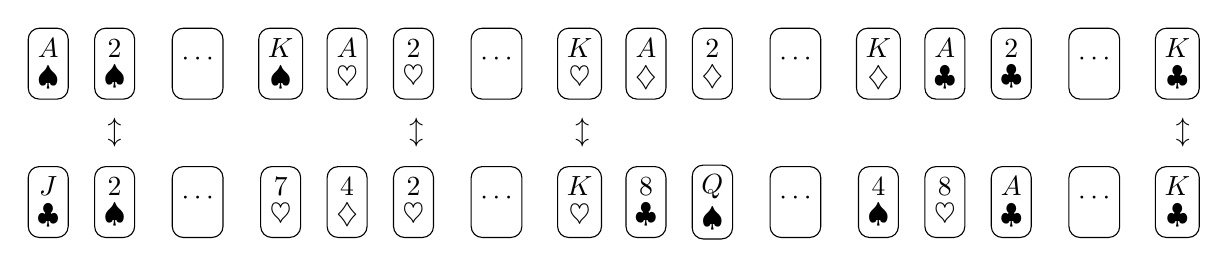
\begin{tikzpicture}
\foreach \x/\v/\s in {
  0/A/\spadesuit,
  1/2/\spadesuit,
  2.25/\cdots/,
  3.5/K/\spadesuit,
  4.5/A/\heartsuit,
  5.5/2/\heartsuit,
  6.75/\cdots/,
  8/K/\heartsuit,
  9/A/\diamondsuit,
  10/2/\diamondsuit,
  11.25/\cdots/,
  12.5/K/\diamondsuit,
  13.5/A/\clubsuit,
  14.5/2/\clubsuit,
  15.75/\cdots/,
  17/K/\clubsuit}
  \node[minimum height=9mm,draw,rounded corners]
    at (\x*24pt,0) {\shortstack{$\v$\\$\s$}};

\foreach \x/\v/\s in {
  0/J/\clubsuit,
  1/2/\spadesuit,
  2.25/\cdots/,
  3.5/7/\heartsuit,
  4.5/4/\diamondsuit,
  5.5/2/\heartsuit,
  6.75/\cdots/,
  8/K/\heartsuit,
  9/8/\clubsuit,
  10/Q/\spadesuit,
  11.25/\cdots/,
  12.5/4/\spadesuit,
  13.5/8/\heartsuit,
  14.5/A/\clubsuit,
  15.75/\cdots/,
  17/K/\clubsuit}
  \node[minimum height=9mm,draw,rounded corners]
    at (\x*24pt,-50pt) {\shortstack{$\v$\\$\s$}};

\node at (24pt,-25pt) {$\updownarrow$};
\node at (133pt,-25pt) {$\updownarrow$};
\node at (193pt,-25pt) {$\updownarrow$};
\node at (410pt,-25pt) {$\updownarrow$};
\end{tikzpicture}
\end{center}
\caption{Matching two decks of cards}\label{f.cards}
\end{figure}
\solution{}

The distribution is uniform because each card in the second row has the same probability of being matched with the card above it. Therefore:
\[
E(\textsf{number of matches}) = 52\cdot \frac{1}{52} = 1\,.
\]

\begin{verbatim}
Expectation of matches = 1.00
Average of matches     = 1.01
\end{verbatim}

%%%%%%%%%%%%%%%%%%%%%%%%%%%%%%%%%%%%%%%%%%%%%%%%%%%%%%%%%%%%%%%%

\begin{prob}{Probabilities of matches\annotate{S}}

Lay out a deck of $n$ cards in a row in the standard order and then lay out a second deck in a row in a random order below the first (Figure~\ref{f.cards}). Develop a formula for $P(n,r)$, the probability that there will be exactly $r$ matches of a card in the first row with the card below? Assume that $P(k,0)$ is given for $0\leq k\leq n$.
\end{prob}
\solution{}

At first glance this problem seems to be related to Problem~28 but there is a major difference. The drawings from the boxes are independent, whereas here the matchings are not independent. For example, if the first match occurs on the first card (with probability $1/n$), the probability that the second card matches is $1/(n-1)$.

The probability that any \emph{given} set of $r$ cards match is:
\begin{equation}\label{eq.r-match}
\disfrac{1}{n}\cdot \disfrac{1}{n-1}\cdot \cdots \cdot \disfrac{1}{n+r-1}\,.
\end{equation}
To obtain exactly $r$ matches Equation~\ref{eq.r-match} must be multiplied by $P(n-r,0)$, the probability that there are no matches in the remaining $n-r$ cards. Finally, there are ${n\choose r}$ ways of choosing the $r$ matches. Therefore:
\begin{eqn}
P(n,r)&=& \dischoose{n}{r}\disfrac{1}{n(n-1)(n+r-1)} P(n-r,0)\\
&=& \disfrac{n!}{r!(n-r)!}\cdot\disfrac{1}{n!/(n-r)!}P(n-r,0)\\
&=&\disfrac{1}{r!}P(n-r,0)\,,
\end{eqn}
which solves the problem since $P(k,0)$ is given.

Mosteller develops a closed formula and a limit for $P(n,r)$:
{
\addtolength{\arraycolsep}{-3pt}
\begin{eqnarray}
\label{eq.r-matches-lim1}
P(n,k)&=&\disfrac{1}{k!}\sum_{i=0}^{n-k} \disfrac{(-1)^i}{i!}\\
\label{eq.r-matches-lim2}
\lim_{n-r\rightarrow \infty} P(n,k)&\approx& \disfrac{1}{k!}e^{-1}\,.
\end{eqnarray}
}
\textbf{Simulation}

The simulation was run for $n=52$ cards and the probability computed from Equation~\ref{eq.r-matches-lim2}.
\begin{verbatim}
Probability of 1 matches = 0.3679
Proportion 1 matches     = 0.3710
Probability of 2 matches = 0.1839
Proportion 2 matches     = 0.1828
Probability of 3 matches = 0.0613
Proportion 3 matches     = 0.0569
Probability of 4 matches = 0.0153
Proportion 4 matches     = 0.0168
\end{verbatim}

%%%%%%%%%%%%%%%%%%%%%%%%%%%%%%%%%%%%%%%%%%%%%%%%%%%%%%%%%%%%%%%%

\begin{prob}{Choosing the largest dowry\annotate{D,S}}
Place $n$ cards in a row face down. There is a positive integer written on the face of each card but you have no knowledge as to their distribution. Turn the cards over one-by-one and look at the numbers. After turning over each card you can declare that it is the largest number. If you are correct you win the game, otherwise you lose. For example, let the sequence of cards be $(47, 23, 55, 4)$. You win only if you choose the third card.

Consider the following strategy: for some fixed $r$ reject the first $r-1$ cards and select the first card whose number is greater than all the $r-1$ cards.

\que{1} For $n=4$ and $r=3$ check all permutations and determine the number of permutations where you win.

\que{2} Develop a formula for the probability of a win for arbitrary $n, r$.

\que{3} Find an approximation for the probability when $n,r\rightarrow \infty$.

\textbf{Hint:} Given $r$ in what positions can the largest number $m$ be and in what positions are numbers less or equal to $m$? 

\end{prob}
\solution{}

\ans{1} 
To simplify notation we write the rank of the numbers as $1,2,3,4$, although the actual numbers are not known, say they are $4,23,47,55$. If you uncover cards $1,2,3$ (which are actually $4,23,47$), you do not know whether to accept $47$ or to reject it and select the last card.

There are $24$ permutations of the four numbers. By the strategy you reject the first two cards and select either the third card or the fourth card, so you lose if the  permutation has $4$ in the first position. What about the permutation $(1,2,3,4)$? You reject $1,2$ and select $3$ since it  greater than $1,2$ but this is not the largest card so you lose. What about the permutation $(1,3,2,4)$? Again, $1,3$ are rejected by the strategy, but $2$ is also rejected because it is \emph{not} larger than $1,3$. Now you select $4$ and win. Carry out this reasoning for all the permutations and check that permutations with boxed $4$s are wins:
\[
\addtolength{\arraycolsep}{-2pt}
\renewcommand*{\arraystretch}{1.5}
\begin{array}{cc|cc@{\hspace{2em}}cc|cc@{\hspace{2em}}cc|cc@{\hspace{2em}}cc|cc@{\hspace{2em}}cc|cc@{\hspace{2em}}cc|cc}
1&2\;&\;3&4&
1&2\;&\;\fbox{4}&3&
1&3\;&\;2&\fbox{4}&
1&3\;&\;\fbox{4}&2&
1&4\;&\;2&3&
1&4\;&\;3&2\\
2&1\;&\;3&4&
2&1\;&\;\fbox{4}&3&
2&3\;&\;1&\fbox{4}&
2&3\;&\;\fbox{4}&1&
2&4\;&\;1&3&
2&4\;&\;3&1\\
3&1\;&\;2&\fbox{4}&
3&1\;&\;\fbox{4}&2&
3&2\;&\;1&\fbox{4}&
3&2\;&\;\fbox{4}&1&
3&4\;&\;2&1&
3&4\;&\;2&1\\
4&1\;&\;2&3&
4&1\;&\;3&2&
4&2\;&\;1&3&
4&2\;&\;3&1&
4&3\;&\;1&2&
4&3\;&\;2&1
\end{array}
\]
The probability of winning is $10/24$.

\ans{2} If the largest number is in one the of positions $1,\ldots,r-1$ you lose. Therefore, in order to win the largest number must be in the $m$th position for $r\leq m\leq n$:
\[
1\quad 2\quad \cdots\quad r-2 \quad r-1 \quad \overbrace{r \quad r+1 \quad \cdots\quad m-1\quad  m \quad m+1\quad \cdots \quad n}^{\textsf{largest number must be here}}\,.
\]
By the strategy you reject the first $r-1$ cards. You will choose position $m$ only if \emph{all} the numbers in $(r,\ldots,m-1)$ are less than \emph{all} the numbers in $(1,\ldots,r)$. In other words, the largest card in the sequence $(1,\ldots,m-1)$ is \emph{not} in the second part of the sequence $(r,\ldots m-1)$ but in the first part $(1,\ldots,r-1)$. The probability is:
\[
P(\textsf{largest card in}\;(1,\ldots,m-1)\;\textsf{is in}\; (1,\ldots,r-1)) = \disfrac{r-1}{m-1}\,.
\]
Since the probability that the largest card is at $m$ is $1/n$:
\begin{equation}\label{eq.dowry1}
P(\textsf{win}) = \sum_{m=r}^{n} \disfrac{1}{n} \cdot \disfrac{r-1}{m-1}= \disfrac{r-1}{n}\sum_{m=r}^{n} \disfrac{1}{m-1}\,.
\end{equation}
For $n=4, r=3$, $P(\textsf{win}) = 5/12=10/24$.

Equation~\ref{eq.dowry1} is not defined for $r=1$ but the probability of winning when choosing the first number is $1/n$. A larger $r$ will have a higher probability of winning as shown in the example.

\ans{3}
Rewrite Equation~\ref{eq.dowry1} as:
\begin{equation}\label{eq.dowry2}
P(\textsf{win}) =\disfrac{r-1}{n}\left(\sum_{m=2}^{n} \disfrac{1}{m-1}-\sum_{m=2}^{r-1} \disfrac{1}{m-1}\right)\,.
\end{equation}
For large $n,r$ Equation~\ref{eq.dowry2} can be approximated by:
\[
P(\textsf{win})=\disfrac{r}{n}(\ln n - \ln r)=\disfrac{r}{n}\ln \disfrac{n}{r}=-\disfrac{r}{n}\ln \disfrac{r}{n}\,.
\]
Denote $x=r/n$ and find the maximum by taking derivatives:
\begin{eqn}
(-x\ln x)' &=& -x\cdot \frac{1}{x} + (-1) \ln x=0\\
\ln x &=& -1\\
x &=& 1/e\,.
\end{eqn}
To maximize that probability of winning choose $r \approx n/e$.

\textbf{Simulation}
The simulation was run with $100$ cards and values of $r$ near $100/e$:
\begin{verbatim}
Reject cards before r = 36:
Probability of wins   = 0.3674
Proportion wins       = 0.3641
Reject cards before r = 37:
Probability of wins   = 0.3678
Proportion wins       = 0.3759
Reject cards before r = 38:
Probability of wins   = 0.3679
Proportion wins       = 0.3548
Reject cards before r = 30:
Probability of wins   = 0.3590
Proportion wins       = 0.3601
\end{verbatim}

%%%%%%%%%%%%%%%%%%%%%%%%%%%%%%%%%%%%%%%%%%%%%%%%%%%%%%%%%%%%%%%%

\begin{prob}{Choosing the largest random number\annotate{D,S}}

Place a sequence of $n$ cards face down. On the face of each card is a real number with uniform distribution in $0.0\leq x<1.0$. Turn the cards over one-by-one and look at the numbers. After turning over each card you can declare that it is the largest number in the sequence. If you are correct you win the game, otherwise you lose.

Use the strategy of Problem~37: decide upon a value $r$ such that you reject the first $r-1$ cards and then select the first card that is larger than the largest value in the first $r-1$ cards.

\textbf{Definition:} $d$, the \emph{indifference value}, is the value below which you decide to reject the card and above which you decide to select the card.

\que{1} Compute $d$ for $n=1$ and compute the probability of winning.

\que{1} Compute $d$ for $n=2$ and compute the probability of winning.

\que{3} Compute $d$ for $n=3$. Do not try to compute the probability of winning!

\textbf{Note:} In Problem~37 the values could be $100, 200, 300$ or $100, 50, 20$ so uncovering the first number gives no information about the other numbers. In this problem, since the distribution is uniform, if the first number is $0.2$, the second number has probability $0.8$ of being larger, and if the first number is $0.8$ the second number has a probability of $0.2$ of being larger.

\end{prob}
\solution{}

Let $v_1,v_2,v_3$ be the values of the three cards.

\ans{1} You have no choice but to select the first card since there are no other cards. There is no indifference value. Since $v_1$ is the ``largest'' number $P({win})=1$.

\ans{2} If you select the first card $P(\textsf{win})=v_1$ which is the probability that the second card has a smaller value. If you reject the first card, $P(\textsf{win})=1-v_1$, which is the probability that $v_2>v_1$. Therefore, if $v_1<0.5$ select the second card because $1-v_1>0.5$ and if $v_1>0.5$ select the first card because $1-v_1<0.5$. It follows that $d=0.5$.

Here is the formula for the probability of winning:
\[
P(\textsf{win}) = p(\textsf{win} \,|\,v_1<0.5)\,p(v_1<0.5)+ p(\textsf{win}\,|\,v_1>0.5)\,p(v_1>0.5)\,.
\]
$p(v_1<0.5)=0.5$ follows by the uniform distribution. What about $p(\textsf{win} \,|\,v_1<0.5)$? By the strategy you win if $0.5<v_2<1$, but you also win if $v_1<v_2<0.5$. Since $v_1$ is uniformly distributed in $(0,0.5)$:
\[
p(\textsf{win} \,|\,v_1<0.5)=\disfrac{1}{2} + \disfrac{1}{4}=\disfrac{3}{4}\,.
\]
A similar computation holds for $v_1>0.5$. Putting the partial computations together gives:
\[
P(\textsf{win})=\disfrac{3}{4}\cdot\disfrac{1}{2}+\disfrac{3}{4}\cdot\disfrac{1}{2}=\disfrac{3}{4}\,.
\]

\ans{3}

If you select the first card $P(\textsf{win})=v_1^2$ because the second and third cards must be smaller than the first.

If you reject the first card and select the second because $v_2>v_1$ then:
\begin{itemize}
\item $P(\textsf{win})=(1-v_1)v_1$ if $v_2>v_1$ and $v_3<v_1$.
\item $P(\textsf{win})=v_1(1-v_1)$ if $v_2<v_1$ and $v_3>v_1$.
\item $P(\textsf{win})=\frac{1}{2}(1-v_1)^2$ if $v_2>v_1$ and $v_3>v_1$, since winning depends on the order: $(0.55, 0.75, 0.65)$ wins and $(0.55, 0.65, 0.75)$ loses.
\end{itemize}

The indifference value $d$ is the value such that the probability of winning by selecting the first card equals the probability of winning by rejecting the first card:
\begin{eqn}
d^2 &=& 2d(1-d) + \frac{1}{2}(1-d)^2\\
5d^2 - 2d -1 &=&0\\
d&=& \disfrac{1+\sqrt{6}}{5}\approx 0.6899\,.
\end{eqn}
Gilbert and Mosteller \cite[page~55]{gilbert} show that for $n=3$:
\[
P(\textsf{win}) = \disfrac{1}{3}+\disfrac{d}{2}+\disfrac{d^2}{1}-\disfrac{3d^3}{2}\approx 0.6617\,.
\]
\textbf{Simulation:}
\begin{verbatim}
For  3 cards:
Indifference value = 0.6000
Probability of win = 0.6693
Proportion of wins = 0.6628
Indifference value = 0.6899
Probability of win = 0.6617
Proportion of wins = 0.6711
Indifference value = 0.7200
Probability of win = 0.6519
Proportion of wins = 0.6473
\end{verbatim}

%%%%%%%%%%%%%%%%%%%%%%%%%%%%%%%%%%%%%%%%%%%%%%%%%%%%%%%%%%%%%%%%
